\documentclass[notitlepage, 12pt]{article}
% package includes
% ---------------------

\usepackage{graphicx} % for include images

\usepackage{url}
\usepackage{caption}
% \usepackage{fullpage}
\usepackage{fancyhdr}
\usepackage{amsmath}
\usepackage{subcaption}
\usepackage{float}
\restylefloat{table}
\restylefloat{figure}
\usepackage{setspace}
% \usepackage{minted}
% \usemintedstyle{colorful}
\graphicspath{{./Pictures/}}

\pagestyle{fancy}
\lhead{Team 4552}
\chead{Problem A}
\rhead{\thepage}

\renewcommand{\headrulewidth}{.8pt}
%\renewcommand{\footrulewidth}{.8pt}

\title{\textbf{Emergency Service Location Optimization in a Multi-Zone County based on Population Distribution}}
\author{Team 4552}

\date{November 15, 2013}

\begin{document}
\maketitle

\tableofcontents

\section{Problem Restatement}
Given a county made up of six separate zones and average travel times between zones, create a model to optimize the placement of $n$ ambulances in order to maximize the number of civilians reached in an eight minute period. Consider the scenarios where $n = 3$, $n = 2$, and $n = 1$, respectively, and for each scenario, keep track of how many people are not being reached with each possible solution.

Then, consider a scenario in which a large scale disaster affects a single location (e.g. the September 11th attacks), and discuss how an Emergency Service Coordinator would cover the situation. Examine how a real-world city or county would prepare for such a disaster. Finally, write a two page memo detailing the model and its analysis for the Emergency Service Coordinator.


\section{Assumptions and Justifications}
\begin{description}
    \item[TODO(drew): Add these assumptions] \hfill \\
    	* Each zone is not a point, but rather a distribution. We experimented with...
        * Route frequency is correlated with population frequency (two random variables?)
    \item[1. Naming] \hfill \\
    	A county is another name for a county. ... TODO(drew)
        Travel...
    \item[2. Zone to Zone Travel] \hfill \\
    	The travel times given are considered to be optimal routes from the center of one zone to
        the center of the another, regardless of any other zones that may lie in between.
    \item[3. Travel Inside Each Zone] \hfill \\
    	The travel times given for travel from any zone to itself is the average
        of all the travel times of the different routes within that zone.
    \item[4. Directional Travel Inside Each Zone] \hfill \\
    	The ratio between the time it takes inside a zone to travel toward a second zone,
        to the time it takes inside a zone to return from a second, is equal to the ratio
        between the travel time from the first zone to the second, and the travel time from the
        second to the first.
    \item[5. Ambulance Placement] \hfill \\
        Ambulances can only be placed in the very center of a zone. Because we do not know the
        spacial position of the zones relative to each other, we cannot consider the ambulances
        being closer to one zone or another.
    \item[6. Partial Coverage] \hfill \\
        Partial ambulance coverage of a zone will be treated as incomplete even coverage over the entire
        zone. Because ambulances of ideal placement are unlikely to overlap in partial coverage, we assume
        that multiple ambulances will cover different areas of the zones, thus evening out coverage.
        (If partial coverages from multiple ambulances sum to above the total population of a zone,
        we assume that zone is completely covered by the ambulances.)
\end{description}

\section{The Model}

\subsection{Model Approach}

Given that a county has $n$ zones, $k$ ambulances need to be placed to maximize the number of people who can be reached in eight minutes or fewer. This system can be represented as a graph of $n$ nodes and $n^2$ vertices. By analyzing all possible configurations, we can identify the ideal nodes to place the ambulances. This algorithm can be made more efficient---albeit less optimal---by employing a greedy heuristic that only focuses on the nodes that provide the most added coverage.

Each zone is a region, and therefore the population is not concentrated on one point. As a result, ambulances will often be able to cover only a fraction of a zone's total population. In order to find these fractions, we developed a model of population density for each zone by extrapolating from the provided average travel times between zones.

Travel time from a zone A to another zone B is not necessarily the same as the travel time in the opposite direction. This inconsistency could be due to a variety of factors, including differences in traffic, roads, and conditions. As a result, these two cases for each pair of zones must be handled separately.

\subsection{Zone-to-Zone Population Dynamics}
An ambulance stationed in one zone may have full, partial, or no coverage of another zone. The population
that the ambulance can cover in a second zone from a first zone (not necessarily distinct),
will be hereafter referred to as zone-to-zone coverage.

A lack of spatial understanding of the county entails the use of a different type of population density. Rather than expressing population as a function of area or distance, we chose to express population density in terms of travel time from a reference point. This is analogous to plotting the number of people a vehicle is likely to meet at each time as it drives along a one-dimensional path.

\begin{figure}
\centering
\begin{subfigure}{.45\textwidth}
  \centering
  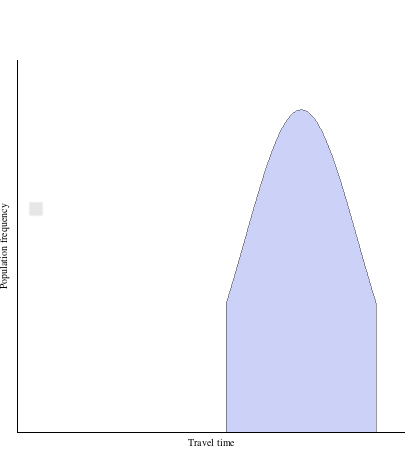
\includegraphics[width=0.9\linewidth]{B(t).png}
  \caption{An example of a zone's population density as a function of travel time from another zone.}
  \label{fig:sub1}
\end{subfigure}%
\hfill
\begin{subfigure}{.45\textwidth}
  \centering
  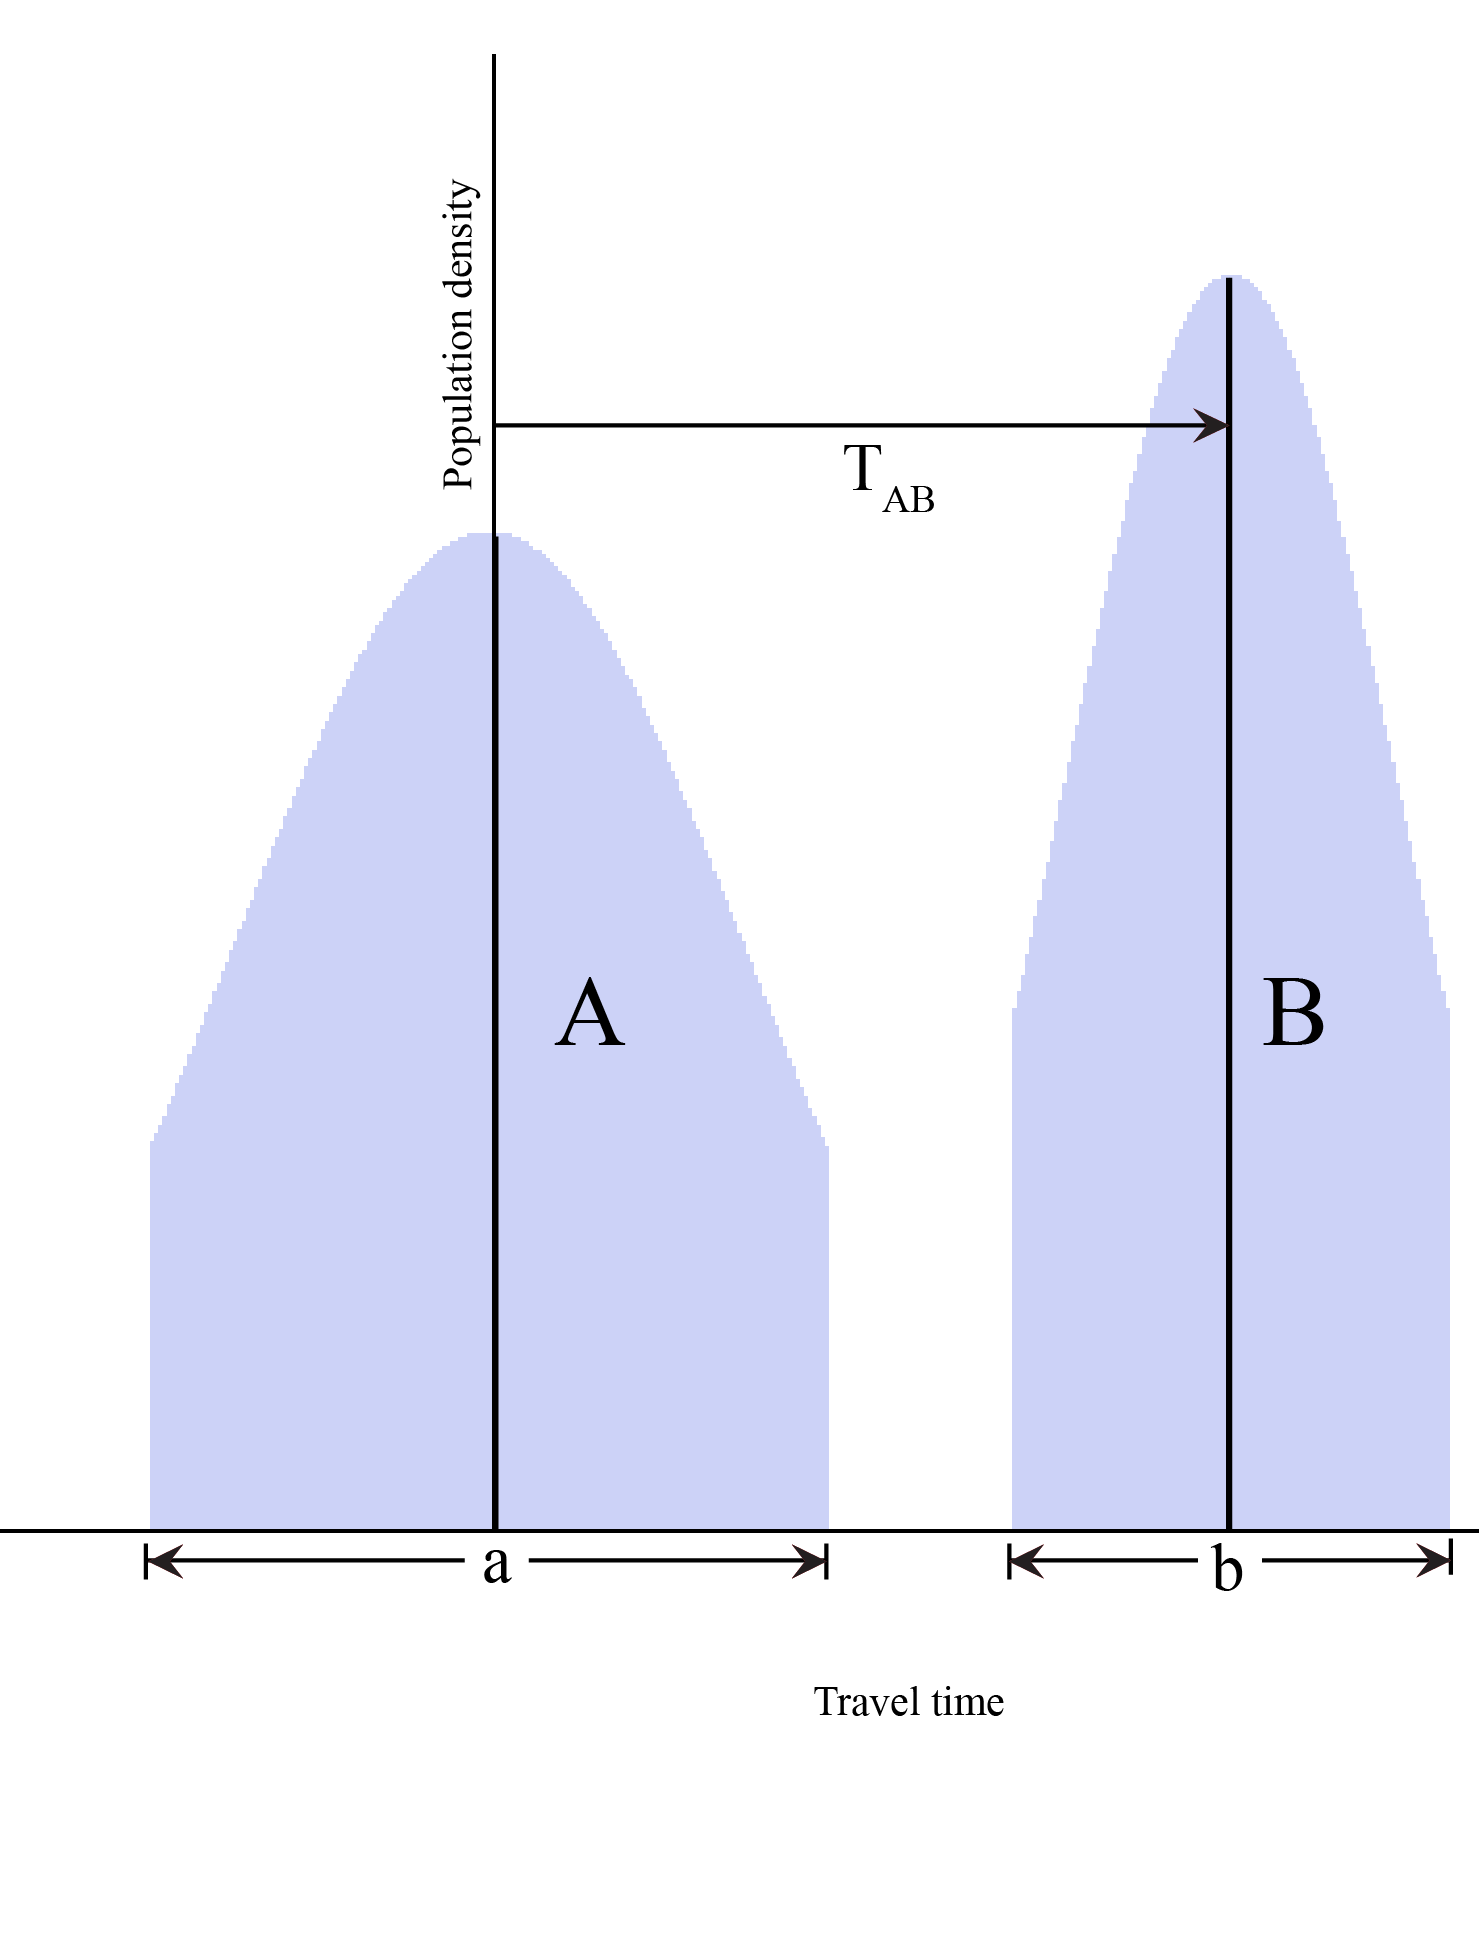
\includegraphics[width=0.9\linewidth]{A(t)B(t).png}
  \caption{TODO(drew)}
  \label{fig:sub2}
\end{subfigure}
\label{fig:test}
\end{figure}

The population that the ambulance can cover in a second zone from a first zone (not necessarily distinct), will be referred to as zone-to-zone coverage.
\newpage

\begin{figure}[htbp]
\begin{center}
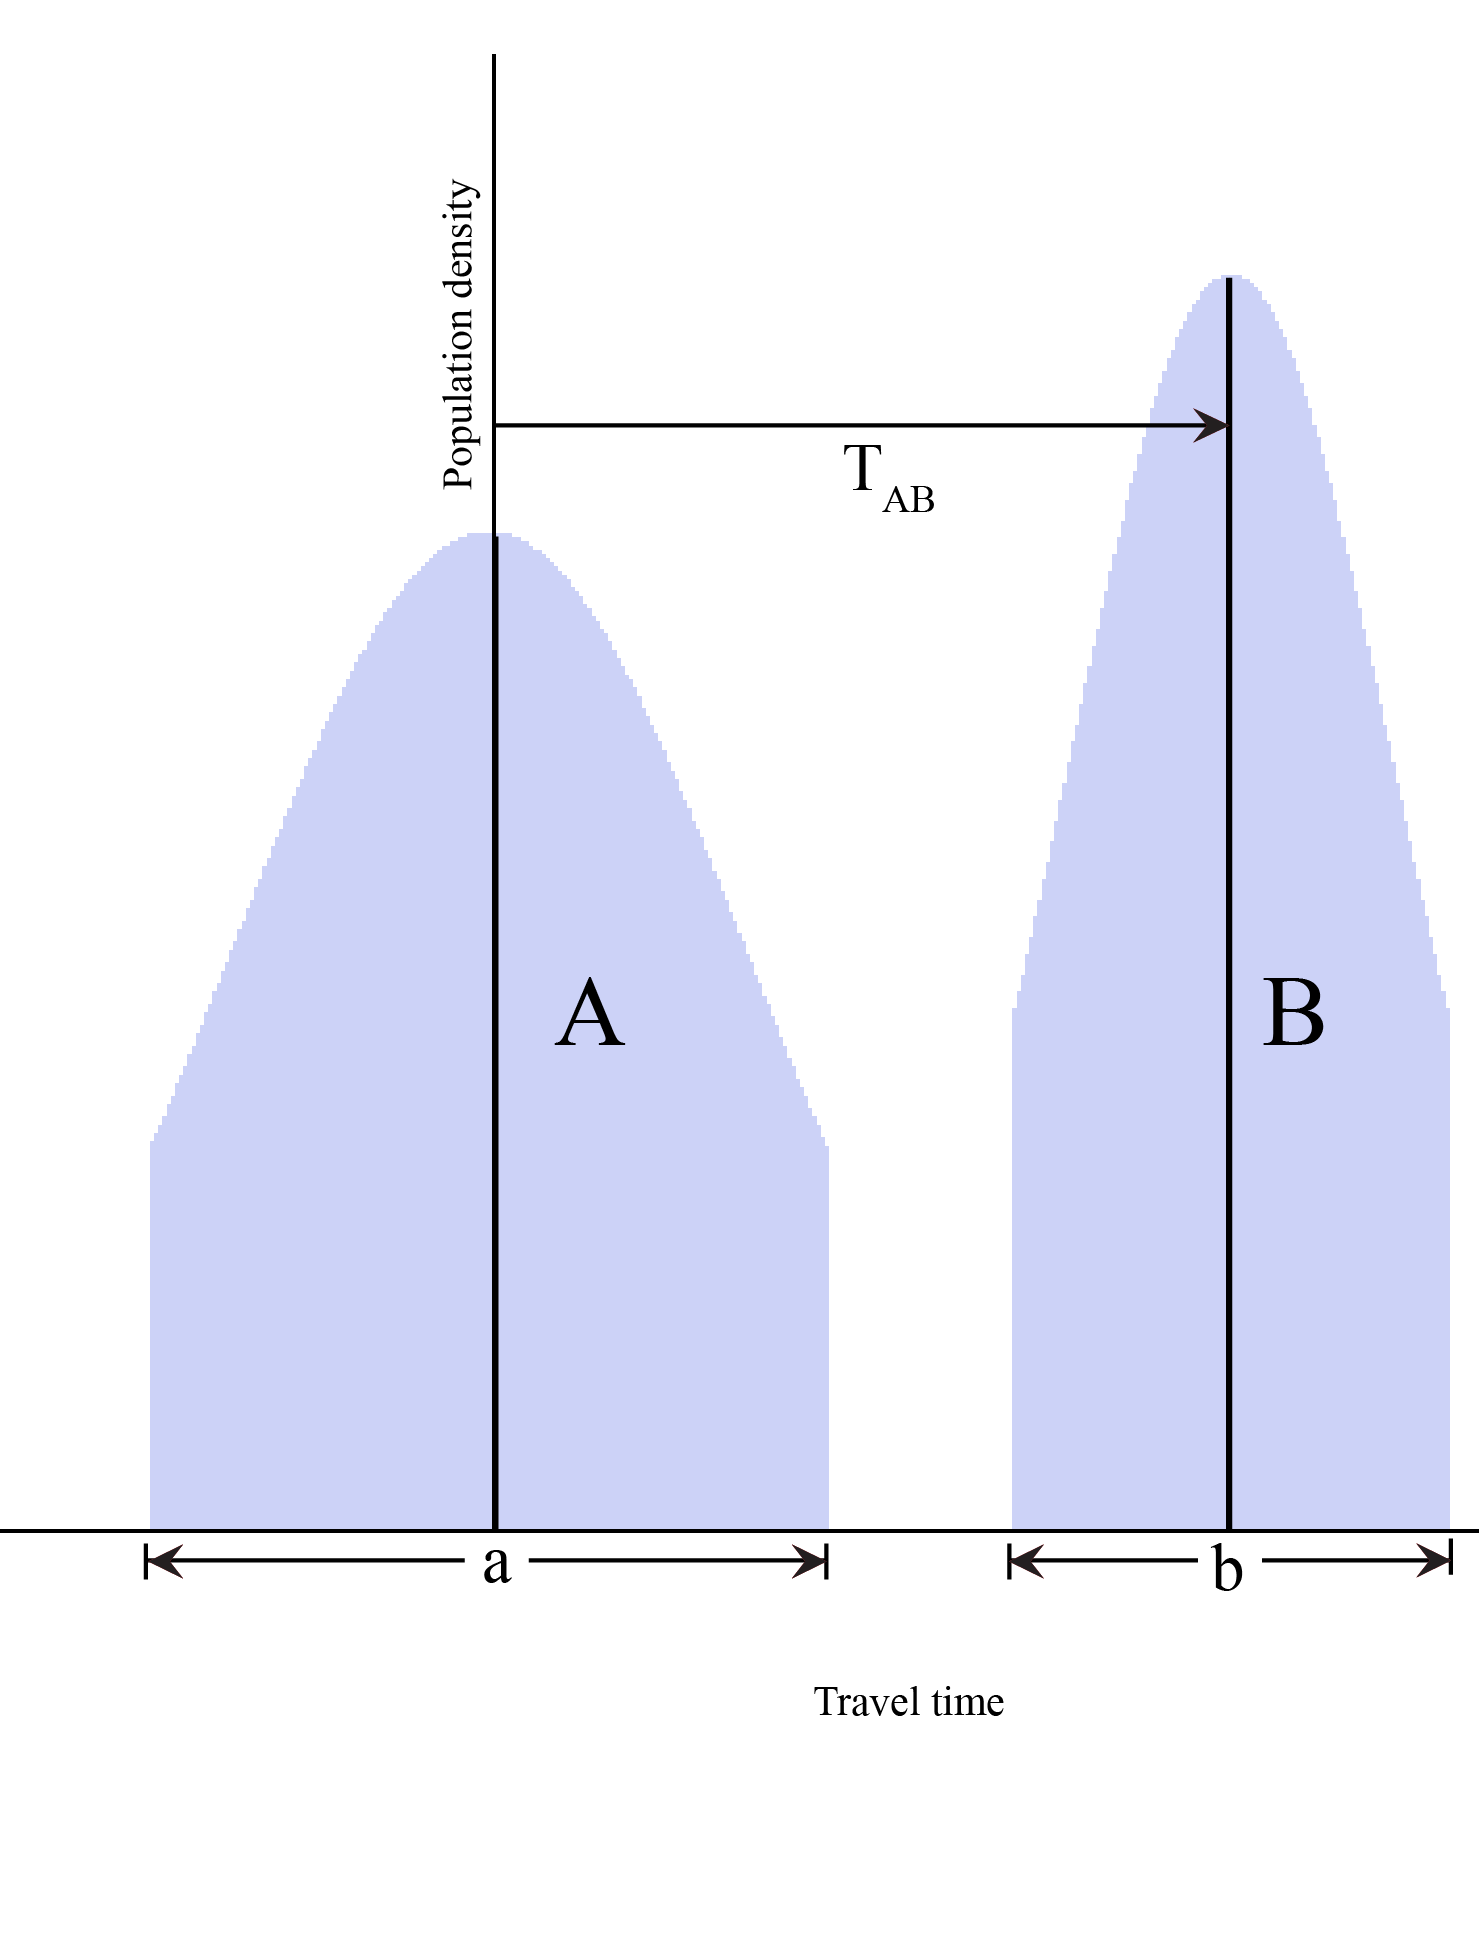
\includegraphics[width=3.5in]{A(t)B(t).png}
\caption{TODO(drew)}
\label{A(t)B(t)}
\end{center}
\end{figure}

\begin{description}
    \item[$\mathbf{A(t), B(t)}$] \hfill \\
    	Zones A and B are two zones separated by a gap. Each zone has a width and a population distribution
    \item[$\mathbf{Z_{AB}(t)}$] \hfill \\
    	Zone-to-zone coverage of B from A
    \item[$\mathbf{v}$] \hfill \\
    	Required ambulance response time
    \item[$\mathbf{T_{AB}}$] \hfill \\
    	Travel time from A to B, given
    \item[$\mathbf{T_{BA}}$] \hfill \\
    	Travel time from B to A, given
    \item[$\mathbf{P_B}$] \hfill \\
    	Total population of B
    \item[$\mathbf{F_B(s)}$] \hfill \\
    	The probability curve for differences in travel time within B
   \item[$\mathbf{T_A}$] \hfill \\
    	Average travel time inside of A
    \item[$\mathbf{T_{A+}}$] \hfill \\
    	Average travel time in the direction of B to A inside of A
    \item[$\mathbf{T_{A-}}$] \hfill \\
    	Average travel time in the direction of A to B inside of A
   \item[$\mathbf{T_B}$] \hfill \\
    	Average travel time inside of B
    \item[$\mathbf{T_{B+}}$] \hfill \\
    	Average travel time in the direction of A to B inside of B
    \item[$\mathbf{T_{B-}}$] \hfill \\
    	Average travel time in the direction of B to A inside of B
    \item[$\mathbf{a, b}$] \hfill \\
    	Width of A and B respectively
    \item[$\mathbf{g}$] \hfill \\
    	Width of the gap between A and B
\end{description}

%TODO: Graphical representation of origin and setup

The function for zone-to-zone coverage in respect to travel time can be written out as
$$Z_{AB}(t) = P_B \int^v_{T_{AB} - \frac{b}{2}} B(t) dt$$

In order to find the width of zone B, b, we can take the probability curve of differences in travel time within B,
$F_B(s)$, and find the average travel time within B. This is the average difference in travel time, and is equal to $T_{B+}$.
$$T_{B+} = \int^{T_{AB} + \frac{b}{2}}_{T_{AB} - \frac{b}{2}} s F_B(s) ds$$

The probability curve of differences in travel time within B, $F_B(s)$, can be found by performing a cross-correlation
of $B(t)$ on itself, with $s$ being the difference in travel time plotted against frequency.
$$P_B(s) =\int^{T_{AB} + \frac{b}{2}}_{T_{AB} - \frac{b}{2}} B(t) * B(t-s) dt$$

The average travel time in the direction of A to B inside of A, $T_{A-}$, and the average travel time in the direction of B to A
inside of A, $T_{A+}$, have a total average travel time of $T_A$. We can also write the ratio of $T_{A+}$ and $T_{A-}$,
which is equivalent to the ratio of $T_{BA}$ and $T_{AB}$. The same can be done with $T_{B}$.
$$T_A = \frac{T_{A+} + T_{A-}}{2}$$
$$\frac{T_{A+}}{T_{A-}} = \frac{T_{BA}}{T_{AB}}$$
$$\frac{T_{B+}}{T_{B-}} = \frac{T_{AB}}{T_{BA}}$$

This allows us to solve for $T_{A-}$  and $T_{B+}$.
$$T_{A-} = \frac {2T_A}{1+ \frac{T_{BA}}{T_{AB}}}$$
$$T_{B+} = \frac {2T_B}{1+ \frac{T_{AB}}{T_{BA}}}$$


\subsection{Ambulance Distribution Optimization}
Once the zone-to-zone coverages have been calculated, we must still decide where to place
the ambulances to maximize total coverage. Total coverage is defined as the sum of the coverages
of the individual zones, i.e. the number of people that can be reached by at least one ambulance
within eight minutes.

Since ambulance placements are assumed to be in the center of zones, putting two ambulances in the same
zone does not increase coverage. Therefore, ambulances should be placed in different zones to maximize
coverage.

Under the given conditions, we can easily find the optimal ambulance placement using a brute force
method: trying all $\binom{6}{3}$ choices of ambulance placements, and picking the one with the highest total coverage.
However, this solution is not scalable to larger cities, as the brute force method has time complexity
$O(n, k) = nk\binom{k}{n}$ where $k$ is the number of zones to cover, and $n$ is the number of ambulances to place, which
becomes intractable as $n$ and $k$ increase (since it has to check $\binom{k}{n}$ placements,
and calculating the total coverage of each placement requires $nk$ computations, summing the $k$ zone-zone
coverages for each of the $n$ ambulances). Quadrupling the size of the city
increases the computations required by a factor of 2 million (assuming the average zone size stays the same,
and the number of ambulances increases proportionally).

Therefore, a more scalable solution is needed. We discovered that a greedy heuristic also gives a good solution,
except with a much lower time complexity of $O(n, k) = n k^2$. The greedy heuristic works by assigning ambulances to zones
one at a time. For each assignment, we iterate through each zone without an ambulance already assigned, and see how many
additional people it would cover; then we assign an ambulance to the zone which would most increase the number of
covered people.

\section{Model Analysis}

\subsection{The $n$ Ambulance Problem}
With the $n$ ambulance problem, we are trying to figure out where to place each of the $n$ ambulances so that the reach of each ambulance covers the most amount of people. For our purposes, this reach is solely determined by how far the ambulance can travel in an eight minute span.

With the given county, made up of six zones, we consider the location optimization under three scenarios; with three ambulances, with two ambulances, and finally, with one ambulance. Our goal is to see a) if we can cover everybody in the county in an eight minute span, and b) if not, how many people are we failing to cover.

The number of people the ambulances are able to cover is a function of our population density function, while the actual location optimization is done by our greedy optimizer.

\subsubsection{$n=3$}

\begin{figure}[htbp]
\begin{center}
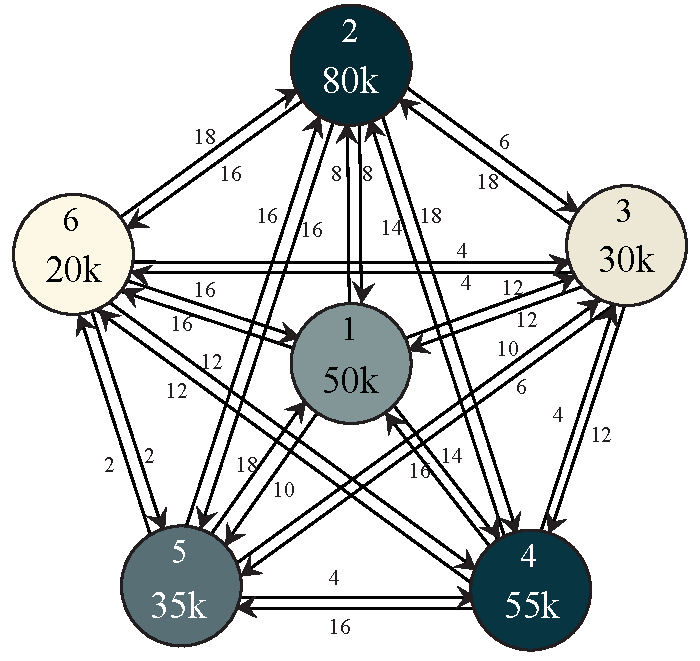
\includegraphics[width=3in]{6point.pdf}
\caption{Graph of zones, populations, and travel times}
\end{center}
\label{fig:fullgraph}
\end{figure}

\begin{figure}[htbp]
\begin{center}
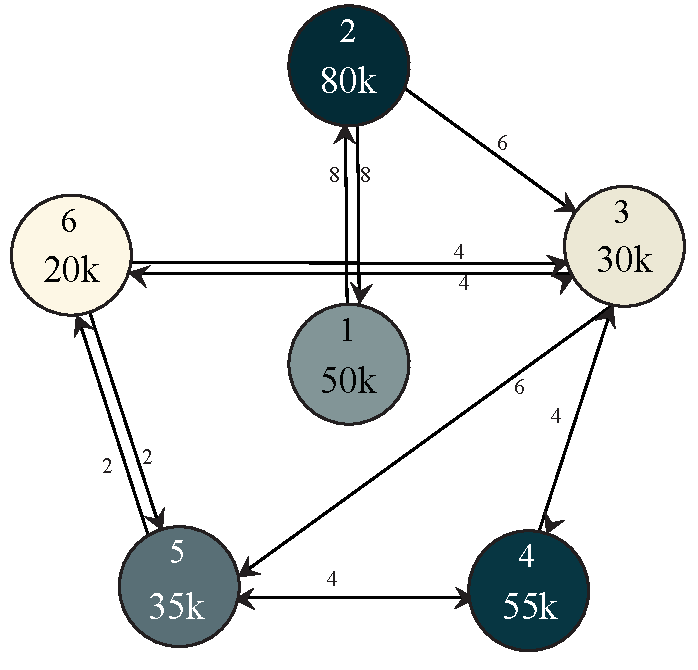
\includegraphics[width=3in]{greedy6point.pdf}
\caption{Graph as in fig. \ref{fig:fullgraph}, with edges longer than 8 minutes removed}
\end{center}
\end{figure}

We ran the greedy algorithm for $n=3$ and we got that ambulances should be placed in zones
2, 3, and 5. This arrangement has ambulances cover all of zones 2-6 and half (25000/50000) of
zone 1.

\subsubsection{$n=2$}
We ran the greedy algorithm for $n=2$ and we got that ambulances should be placed in zones
2 and 5. This arrangement has ambulances cover all of zones 2, 4-6, half (25000/50000) of
zone 1, and none of zone 3.

\subsubsection{$n=1$}
We ran the greedy algorithm for $n=1$ and we got that our ambulance should be placed in zone 5. This arrangement allows the single ambulance to cover all of zone 4-6.

\subsection{Localized Single Zone Disaster}
In a localized catastrophic event such as those that happened on September 11, 2001, there will be
many casualties in a single location that require aid. Ambulances, and other emergency vehicles,
such as police cars and fire trucks, will need to respond quickly in order to aid the most critically
injured first, who will be sorted by triage \cite{ColRev}. Therefore, it is very important for ambulances to be able to
reach the emergency as quickly as possible, regardless of the initial location of the ambulances and the
location of the emergency.

Catastrophic events will cause more casualties than emergency personnel will be able to service, so as a result,
ambulances will have to act as shuttles to hospitals for the injured. Therefore, to maximize throughput
cities should arrange hospitals to minimize the average time between all areas and the nearest
hospital.

Since metropolitan areas are most likely to be affected by catastrophic events, and catastrophic events there
will affect significantly more people, to maximize patient throughput cities should arrange hospitals to minimize
the average time between all areas and the nearest hospital. Futhermore, due to differences in population density,
statistically, an accident in a metropolitan area will demand more urgent care than a similar accident
in a rural or suburban area. Therefore, when the city lays out its stations for ambulances, attempting to minimize
travel times to any area, it should put significantly more weight on minimizing travel time to metropolitan areas.

\section{Strengths and Weaknesses}

\begin{table}[H]
    \centering
    \begin{tabular}{ p{6.25cm}|p{6.25cm} }
        \textbf{Strengths} & \textbf{Weaknesses}\\
        \hline
        1. Our model, by virtue of its polynomial-time greedy selection algorithm, is extremely scalable. We can scale up to large datasets, consisting of many, larger zones. Also, because of a non-exponential time algorithm, our model is also extremely efficient. & 1. Because of the greedy nature of our algorithm, we are not guaranteed to find the optimal solution for the location of the ambulances.\\
        2. Our model is also adaptable to various different population distributions. Population Distributions can vary with the addition of any new data. The more accurate the data, the more accurate the model becomes. & 2. In order to find the optimal solution, our brute force optimizer works in exponential time, so at a large scale, finding the optimal placement of ambulances is near impossible. \\
        3. Completely flexible model. Depending on any number of nodes, any number of ambulances, and any population distribution, we will be able to find a good answer relatively quickly.

    \end{tabular}
    \caption{Model Strengths \& Weaknesses}
    \label{tab:modelprocons}
\end{table}


\section{Extensions}
Though our model performs fairly well already, providing us with the optimal locations of our $n$ ambulances to
maximize the number of people saved, there are a number of ways we can improve the model so that we can make more
accurate predictions as to the number of people we can reach in an eight minute period. Furthermore, we can also
improve the overall efficiency of the solution algorithm itself, by looking at potential dynamic programming approaches to the problem.

While any algorithmic changes may not be necessary with only six zones, and a maximum of $n = 3$ ambulances, if
we scale this problem up to a large city, or across multiple counties, algorithm efficiency becomes an important problem that requires attention.

\subsection{Population Distribution}
As it currently stands, we have very little information regarding the actual population distribution of each
zone in the scope of the county, which provides us with a slightly skewed perception. While we justified the
use of a standard distribution for population above, we have the ability to greatly improve our model with a
better idea of how spread out a population of a zone actually is, in relation to its epicenter. This information
allows us to better predict how many people an ambulance would miss (not be able to cover) in a certain zone.

The number of missed people is an important statistic that an Emergency Service Coordinator needs to have in
order to fully optimize their resources. In our system now, we predict this number with a certain level of accuracy,
but we are still prone to a relatively large amount of error. With a better understanding of the population and
geospatial makeup of each individual zone, we would be able to better optimize our resources and potentially save more people.

\subsection{Dynamic Approach}
With only a total of six zones and a maximum of $n = 3$ ambulances to allocate, overall algorithm efficiency is
not a pressing issue. As we have shown above, even a brute force attempt at optimizing the ambulance locations
takes a negligible amount of time. However, as we look to expanding the model to fit a larger area, with more
zones, and more ambulances, it becomes increasingly more important to look for ways to make our algorithm more efficient.

Even after our greedy algorithm reduces the overall solution time to an $O(n, k) = nk^2$, or polynomial time, there
are still possible ways to improve it. One such method would be the use of dynamic programming methods to split the
problem up into a series of smaller subproblems, and then merge the results together. As a result of such a method,
we would reduce the problem to one with an $O(n, k) = nk\log(k)$, an algorithm that would easily scale to larger data sets.

However, the implementation of such a method is slightly less simple.
One such way to implement a solution in this manner would be in the following fashion:

\begin{enumerate}
\item Given a graph of each node (zone), and the edges between them (time it takes to travel between nodes),
    immediately remove all infeasible edges, with edge length (time) greater than the eight minute baseline.

\item Identify a set of nodes such that there is a large number of outgoing edges, thereby identifying potential
    split points, to divide each county into smaller sub-counties. Make sure to account for overlap.

\item Allocate $n$ ambulances across the sub-counties. If there are fewer ambulances than are necessary to cover
    the entire county, weight each sub-county by population size (save more people per ambulance).

\item Solve each sub-county for the optimal ambulance location, thereby finding a solution for the set as a whole.
\end{enumerate}

While we are not guaranteed to find the optimal solution to ambulance location, we will be provided with a relatively
good one, in a short amount of time. There are tradeoffs to using such a model, but especially at a large scale,
this methodology is realistically the one an Emergency Service Coordinator would use.

\section{Non-Technical Memo}

\newpage
\appendix
\section{Code}
The following contains the code for both our brute force location optimizer, as well as the greedy optimizer. Both functions take a parameter $nambulances$, representing the total number of ambulances we have to allocate across the county.

% \inputminted[fontsize=\footnotesize]{python}{../Code/optimizer.py}




\bibliographystyle{unsrt}
\bibliography{references}
\end{document}
